
\documentclass{article}


\usepackage[utf8]{inputenc}
\usepackage[a4paper, total={6in, 9in}]{geometry}
\usepackage{braket}
\usepackage{xcolor}
\usepackage{amsmath}
\usepackage{amsfonts}
\usepackage{tikz}
\usepackage{svg}
\usepackage{graphicx}
\usepackage{media9}
\usepackage{float}
\usetikzlibrary{calc}
\usepackage{array}
\usepackage[ruled,vlined,linesnumbered]{algorithm2e}

\usepackage[
backend=biber,
style=alphabetic,
sorting=ynt
]{biblatex}



\newcommand{\commentt}[1]{\textcolor{blue}{ \textbf{[COMMENT]} #1}}
\newcommand{\ctt}[1]{\commentt{#1}}
\newcommand{\prb}[1]{ \mathbf{Pr} \left[ {#1} \right]}
\newcommand{\onotation}[1]{\(\mathcal{O} \left( {#1}  \right) \)}
\newcommand{\ona}[1]{\onotation{#1}}
\newcommand{\nvar}[2]{ \( #1_{1}, #1_{2} ... #1_{#2}  \) }
%\newenvironment{proof}[0]{\paragraph{Proof.}}{}
%\newenvironment{remark}[0]{\textit{remark}}{}
\newenvironment{cor}[0]{\paragraph{Corollary.}}{}
\newenvironment{example}[0]{\paragraph{Example.}}{}
%\newenvironment{thm}[0]{\paragraph{Theorem.}}{}
\newtheorem{prop}{Proposition}
\newtheorem{ex}{Exercise}
\newtheorem{sol}{Solution}
\newtheorem{theorem}{Theorem} 		
\newtheorem{thm}{Theorem}[section]
\newtheorem{conj}[thm]{Conjecture} 	
\newtheorem{lemma}[thm]{Lemma}
\newtheorem{corollary}[thm]{Corollary} 
\newtheorem{claim}[thm]{Claim}
\newtheorem{proposition}[thm]{Proposition}
\newtheorem{definition}{Definition} 
\newtheorem{remark}{Remark}
 


% \addbibresource{sample.bib} %Import the bibliography file
\begin{document}    
\maketitle
\newcommand{\image}{\text{ Im } }


\begin{document}
\ifdefined\BOOK
\else
\setcounter{chapter}{8}
\fi

\chapter{Graphs}

\usetikzlibrary{positioning, arrows}
\tikzset{main node/.style={circle,draw,minimum size=0.8cm,inner sep=0pt},}
\tikzset{edge/.style = {->,> = latex'}}

\iffalse
%\newtheorem{prop}{Proposition}
%\newtheorem{ex}{Exercise}
%\newtheorem{sol}{Solution}
%\newtheorem{theorem}{Theorem} \newtheorem{thm}{Theorem}[section]
%\newtheorem{conj}[thm]{Conjecture} \newtheorem{lemma}[thm]{Lemma}
%\newtheorem{corollary}[thm]{Corollary} \newtheorem{claim}[thm]{Claim}
%\newtheorem{proposition}[thm]{Proposition}
%\newtheorem{definition}{Definition} \newtheorem{remark}{Remark}
   
%\pagestyle{empty}

%\setlength{\textwidth}{6.5in}
%\setlength{\evensidemargin}{0.0in}
%\setlength{\oddsidemargin}{0.0in}
%\setlength{\topmargin}{-0.25in}
%\setlength{\textheight}{9.0in}
%\setlength{\baselineskip}{1.3\baselineskip}
%\setlength{\parindent}{.0in}
\fi
\tikzset{
node of list/.style = { 
             draw, 
             fill=orange!20, 
             minimum height=6mm, 
             minimum width=6mm,
             node distance=6mm
   },
link/.style = {
     -stealth,
     shorten >=1pt
     },
array element/.style = {
    draw, fill=white,
    minimum width = 6mm,
    minimum height = 10mm
  }
}

\def\LinkedList#1{%
  \foreach \element in \list {
     \node[node of list, right = of aux, name=ele] {\element};
     \draw[link] (aux) -- (ele);
     \coordinate (aux) at (ele.east);
  } 
}



%%%%%%%%%%%%%%%%%%%%%%%%%%%%%%%%%%%%%%%%%%%%%%%%%%%%%%%%%%%%



%%%%%%%%%%%%%%%%%%%%%%%%%%%%%%%%%%%%%%%%%%%%%%%%%%%%%%%%%%%%

%\vspace{0.2in}

\section{Graphs}
This is an important section, as you'll see graphs A LOT in this course and in the courses to follow. 

\subsection{Definitions, Examples, and Basics}

\begin{figure}[h]
\begin{subfigure}[b]{0.65\textwidth}
\begin{definition}
A \textbf{non-directed graph} $G$ is a pair of two sets - $G=(V, E)$ - $V$ being a set of vertices and $E$ being a set of couples of vertices, which represent edges ("links") between vertices.
\end{definition}

\textbf{Example}: $G= (\{1,2,3,4\},\ \{\{1,2\}, \{1,3\}, \{3,4\}\})$ is the following graph:\\ 
\end{subfigure}
\begin{subfigure}[b]{0.05\textwidth}
  \
\end{subfigure}
  \begin{subfigure}[b]{0.25\textwidth}
    \begin{tikzpicture}
\node[main node](1){$1$};
\node[main node](2)[below = 1cm of 1]{$2$};
\node[main node](3)[right = 1cm of 1]{$3$};
\node[main node](4)[below = 1cm of 3]{$4$};

\path[draw, thick]
(1) edge node {} (2)
(1) edge node {} (3)
(3) edge node {} (4);
\end{tikzpicture}
\end{subfigure}
\end{figure}
\begin{figure}[h]
\begin{subfigure}[b]{0.65\textwidth}
\begin{definition}
A \textbf{directed graph} $G$ is a pair of two sets - $G=(V, E)$ - $V$ being a set of vertices and $E\subseteq V\times V$ being a set of directed edges ("arrows") between vertices.
\end{definition}
\textbf{Example}: $G=(\{1,2,3,4\},\ \{(1, 2), (1, 4), (4, 1), (4,3)\})$ is the following graph (note that it has arrows): \\ 
\end{subfigure}
\begin{subfigure}[b]{0.05\textwidth}
  \
\end{subfigure}
  \begin{subfigure}[b]{0.25\textwidth}
    \begin{tikzpicture}
\node[main node](1){$1$};
\node[main node](2)[below = 1cm of 1]{$2$};
\node[main node](3)[right = 1cm of 1]{$3$};
\node[main node](4)[below = 1cm of 3]{$4$};

\draw[edge] (1) to (2);
\draw[edge] (1) to (4);
\draw[edge] (4) to (1);
\draw[edge] (4) to (3);
\end{tikzpicture}
\end{subfigure}
\end{figure}

\begin{definition}
  A \textbf{weighted graph} composed by a graph $G=\left( V,E \right)$ (either non-directed or directed) and a weight function $w : E \rightarrow \mathbb{R}$. Usually (but not necessary), we will think about the quantity $w(e)$, where $e \in E$, as the length of the edge.  
\end{definition}

Now that we see graphs with our eyes, we can imagine all sorts of uses for them... For example, they can represent the structure of the connections between friends on Facebook, or they can even represent which rooms in your house have doors between them.

\begin{remark}
Note that directed graphs are a \textbf{generalization} of non-directed graphs, in the sense that every non-directed graph can be represented as a directed graph. Simply take every non-directed edge $\{v,u\}$ and turn it into two directed edges $(v,u), (u,v)$. 
\end{remark}

\begin{remark}
Note that most of the data structures we discussed so far - Stack, Queue, Heap, BST - can all be implemented using graphs.
\end{remark}

Now let's define some things in graphs:

\begin{definition} (Path, circle, degree)
\begin{enumerate} 
\item A \textbf{simple path} in the graph $G$ is a series of unique vertices (that is, no vertex appears twice in the series) $v_1, v_2, ..., v_n$ that are connected with edges in that order. 
\item A \textbf{simple circle} in the graph $G$ is a simple path such that $v_1 = v_n$. 
\item The \textbf{distance} between two vertices $v,u\in V$ is the length of the shortest path between them ($\infty$ if there is no such path).
\end{enumerate}
\end{definition}

\begin{remark}
Note that for all $u,v,w\in V$ the triangle inequality holds regarding path lengths. That is:
$$dist(u,w)\leq dist(u,v) + dist(v, w)$$
\end{remark}

\begin{definition} (connectivity)
\begin{enumerate}
  \item Let $ G =\left( V,E \right)$ be a non-directed graph. A \textbf{connected component} of $G$ is a subset $U \subseteq V$ of maximal size in which there exists a path between every two vertices. 
\item A non-directed graph $G$ is said to be a \textbf{connected} graph if it only has one connected component.
\item Let $ G = \left(V, E\right)$ be a directed graph. A \textbf{strongly connected component} of $G$ is a subset $U \subseteq V$ of maximal size in which for any pair of vertices $u,v \in U$ there exist both directed path from $u$ to $v$ and a directed path form $v$ to $u$.   
\end{enumerate}
\end{definition}
%\begin{figure}[h]
  %\begin{subfigure}[b]{0.4\textwidth} 
%An \textbf{example} of a non-connected graph: \\ \\ \\  \\
%\end{subfigure}
%\begin{subfigure}[b]{0.05\textwidth}
  %\
%\end{subfigure}
%\begin{subfigure}[b]{0.25\textwidth}
%\begin{tikzpicture}
%\node[main node](1){$1$};
%\node[main node](2)[below = 1cm of 1]{$2$};
%\node[main node](3)[right = 1cm of 1]{$3$};
%\node[main node](4)[below = 1cm of 3]{$4$};
%
%\draw[edge] (1) to (2);
%\draw[edge] (3) to (4);
%\end{tikzpicture}
%\end{subfigure}
%\end{figure}

\begin{claim}
Let $G=(V,E)$ be some graph. If $G$ is connected, then $|E| \geq |V|-1$
\end{claim}

\begin{proof}
We will perform the following process: Let $\{e_1,...,e_m\}$ be an enumeration of $E$, and let $G_0=(V,\emptyset)$. We will build the graphs $G_1, G_2,... G_m=G$ by adding edges one by one. Formally, we define - 
$$\forall i\in[m]\ \ G_i=(V,\{e_1,...,e_i\})$$
$G_0$ has exactly $|V|$ connected components, as it has no edges at all. Then $G_1$ has $|V|-1$. From there on, any edges do one of the following:
\begin{enumerate}
    \item Keeps the number of connected components the same (the edge closes a cycle)
    '\item Lowers the number of connected components by $1$ (the edges does not close a cycle)
\end{enumerate}

So in general, the number of connected components of $G_i$ is $\geq |V|-i$. 
Now, if $G_m=G$ is connected, it has just one connected component! This means:
$$1 \geq |V| - |E|\ \implies \ |E|\geq|V|-1$$

\end{proof}


\subsection{Graph Representation}

Okay, so now we know what graphs are. But how can we represent them in a computer? There are two main options. The first one is by \textbf{array of adjacency lists}. Given some graph $G$, every slot in the array will contain a linked list. Each linked list will represent a list of some node's neighbors. The second option is to store edges in an \textbf{adjacency matrix}, a $ |V| \times |V| $ binary matrix in which the $v,u$-cell equals $1$ if there is an edge connecting $u$ to $v$. That matrix is denoted by $A_{G}$ in the example below. Note that the running time analysis might depend on the underline representation.     

\textbf{Question.} What is the memory cost of each of the representations? Note that while holding an adjacency matrix requires storing $|V|^2$ bits regardless of the size of $E$, Maintaining the edges by adjacency lists costs linear memory at the number of edges and, therefore, only $ \Theta \left(  |V| + |E| \right) $ bits. 

\paragraph{Example.} Consider the following directed graph:
\begin{figure}[h]
  \centering
  \begin{subfigure}[b]{0.25\textwidth}
    \begin{tikzpicture}
      \node[main node](1){$1$};
      \node[main node](2)[below = 1cm of 1]{$2$};
      \node[main node](3)[right = 1cm of 1]{$3$};
      \node[main node](4)[below = 1cm of 3]{$4$};

      \draw[edge] (1) to (2);
      \draw[edge] (1) to (4);
      \draw[edge] (4) to (1);
      \draw[edge] (4) to (3);
      \draw[edge] (1) to (3);
      \draw[edge] (3) to (1);
    \end{tikzpicture}  
    \\ \\  
  \end{subfigure} 
  \begin{subfigure}[b]{0.49\textwidth}
    \begin{tikzpicture}
      \foreach \index/\list in {1/{2,3,4,null}, 2/{null}, 3/{1, null}, 4/{1, 3, null}} {
	\node[array element] (aux) at (0,-\index) {\index};
	\LinkedList{\list}
      }
    \end{tikzpicture}  
  \end{subfigure}
  \caption{ Persenting $G$ by array of adjacency lists.  }
\end{figure}

%Its representation will be: \\ \\

\begin{figure}[h]
  \centering
  \begin{subfigure}[b]{0.25\textwidth}
        \begin{tikzpicture}
\node[main node](1){$1$};
\node[main node](2)[below = 1cm of 1]{$2$};
\node[main node](3)[right = 1cm of 1]{$3$};
\node[main node](4)[below = 1cm of 3]{$4$};

\draw[edge] (1) to (2);
\draw[edge] (1) to (4);
\draw[edge] (4) to (1);
\draw[edge] (4) to (3);
\draw[edge] (1) to (3);
\draw[edge] (3) to (1);
\end{tikzpicture} \\ 
  \end{subfigure}
\begin{subfigure}[b]{0.49\textwidth}       
  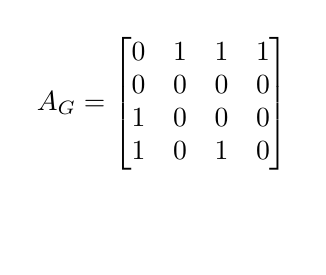
\begin{tikzpicture}
    \node (1) at (0,0) { };
    \node  (2) at (1,1.7) { $ A_{G} = 
	  \begin{bmatrix}
	0 & 1 & 1 & 1\\
	0 & 0 & 0 & 0\\
	1 & 0 & 0 & 0\\
	1 & 0 & 1 & 0
	\end{bmatrix}
      $ };
      \end{tikzpicture}
\end{subfigure}
\caption{ Presenting $G$ by adjacency matrix. }
\end{figure}

\subsection{Breadth First Search (BFS)}

One natural thing we might want to do is to travel around inside a graph. That is, we would like to visit all of the vertices in a graph in some order that relates to the edges. 
Breadth-first search constructs a breadth-first tree, initially containing only its root, which is the source vertex $s$. Whenever the search discovers a white vertex $v$ in the course of scanning the adjacency list of a gray vertex $u$, the vertex $v$ and the edge ($u$, $v$) are added to the tree. We say that $u$ is the predecessor or parent of $v$ in the breadth-first tree. Since every vertex reachable from $s$ is discovered at most once, each vertex reachable from $s$ has exactly one parent. (There is one exception: because $s$ is the root of the breadth-first tree, it has no parent.) Ancestor and descendant relationships in the breadth-first tree are defined relative to the root $s$ as usual: if $u$ is on the simple path in the tree from the root $s$ to vertex $v$, then $u$ is an ancestor of $v$, and $v$ is a descendant of $u$.
The breadth-first-search procedure BFS on the following page assumes that the graph $G = (V, E)$ is represented using adjacency lists. It denotes the queue by $Q$, and it attaches three additional attributes to each vertex $v$ in the graph:

\begin{enumerate}
    \item $v$.visited is a boolean flag which indicate wheter $v$ was allready visited.
    \item $\pi(v)$ is $v$’s predecessor in the breadth-first tree. If $v$ has no predecessor because it is the source vertex or is undiscovered, then $\pi(v)$ is None/NULL.
\end{enumerate}

  \begin{algorithm}[H]
  \caption{BFS($G, s$)}
    \For {$v\in V$}{
	 $v.visited \leftarrow $ False 
     }
 $Q\leftarrow$ new Queue \\ 
 $Q$.Enqueue($s$) \\
 $s$.visited $\leftarrow$ True \\
 \While {$Q$ is not empty} {
 $u\leftarrow Q$.Dequeue() \\
	\For {neighbor $w$ of $u$} {
	\If {$w$.visited is False}{
		 $w$.visited$\leftarrow$ True \\
		 $\pi(w) \leftarrow u $ \\
		 $Q$.Enqueue($w$)

	      }
	}
      }
  \end{algorithm}

\underline{Correctness}: The example should be enough to explain the correctness. A concrete proof can be found in the book, page 597.

\underline{Runtime}: We can analyse the runtime line-by-line:
\begin{itemize}
\item Lines 1-2: $|V|$ operations, all in $O(1)$ runtime, for a total of $O(|V|)$.
\item Lines 3-6: $O(1)$
\item Lines 7-8: First we need to understand the number of times the $while$ loop iterates. We can see that every vertex can only enter the queue ONCE (since it is then tagged as "visited"), and therefore it runs $\leq |V|$ times. All operations are $O(1)$, and we get a total of $O(|V|)$. 
\item Lines 9-13: Next, we want to understand the number of times this $for$ loop iterates. 
The for loop starts iterating once per vertex, and then the number of its iterations is the same as the number of neighbors that this vertex has. Thus, it runs $O(|E|)$ times.
\end{itemize}
So all in all we get a runtime of $O(|V|+|E|)$

\subsection{Usage of BFS}
Now we have a way to travel through a graph using the edges. How else can we use it?\\ \\ 
\textbf{Exercise}: Present and analyse an algorithm $CC(G)$ which receives some undirected graph $G$ and outputs the number of connected components in $G$ in $O(|V|+|E|)$. \\

\textbf{Solution}: Consider the following algorithm: 

  \begin{algorithm}[H]
  \caption{CC($G$)}
     count $\leftarrow 0$\\
     \For {$v\in V$ }{
	\If {$v$.visited = False} {
	  count$\leftarrow$count$+1$ \\
	  BFS($G, v$)
	}
      }
	\Return count
  \end{algorithm}

\subsection{Depth First Search (DFS)}
As its name implies, depth-first search searches "deeper" in the graph whenever possible. Depth-first search explores edges out of the most recently discovered vertex $v$ that still has unexplored edges leaving it. Once all of $ v$'s edges have been explored, the search "backtracks" to explore edges leaving the vertex from which $v$ was discovered. This process continues until all vertices that are reachable from the original source vertex have been discovered. If any undiscovered vertices remain, then depth-first search selects one of them as a new source, repeating the search from that source. The algorithm repeats this entire process until it has discovered every vertex.

  \begin{algorithm}[H]
  \caption{DFS($G$)}
   \bf{DFS}( $G$): \\
    \For {$v\in V$}{
 	$vi$.visited $\leftarrow False$
    }
    time $ \leftarrow 1 $\\
    \For {$v\in V$}{
      \If { not $v$.visited } {
	$\pi \left( v \right)  \leftarrow $ null \\ 
	Explore( $G,v$ ) 
     } 
   }

  \end{algorithm}

  \begin{algorithm}[H]
    \bf{Explore}($G,v$): \\
     Previsit($v$)
    \For {$\left( v,u \right) \in E  $}{
      \If { not $u$.visited } {
	$ \pi \left( u \right) \leftarrow v $ \\ 
	Explore( $G, u$ ) 
      }
    }
    Postvisit($v$)
  \end{algorithm}
  \begin{algorithm}[H]
    \bf{Previsit}($v$): \\
    pre($v$) $\leftarrow $ time \\
    time $\leftarrow$ time $+1$
  \end{algorithm}
 \begin{algorithm}[H]
   \bf{Postvisit} ($v$): \\ 
    post($v$) $\leftarrow $ time \\
    time $\leftarrow$ time $+1$
  \end{algorithm}


\paragraph{Properties of depth-first search.} Depth-first search yields valuable information about the structure of a graph. Perhaps the most basic property of depth-first search is that the predecessor subgraph $G_{\pi}$ does indeed form a forest of trees since the structure of the depth-first trees exactly mirrors the structure of recursive calls of explore-function. That is, $u$ = $\pi\left( v \right)$ if and only if explore($G, v$) was called during a search of $ u$'s adjacency list. Additionally, vertex $v$ is a descendant of vertex $u$ in the depth-first forest if and only if $v$ is discovered during the time in which $u$ is gray.
Another important property of depth-first search is that discovery and finish times have a parenthesis structure. If the explore procedure were to print a left parenthesis "$(u$" when it discovers vertex $u$ and to print a right parenthesis r``$u)$" when it finishes $u$, then the printed expression would be well-formed in the sense that the parentheses are properly nested.

The following theorem provides another way to characterize the parenthesis structure.

\paragraph{Parenthesis theorem}
In any depth-first search of a (directed or undirected) graph $G = (V, E)$, for any two vertices $u$ and $v$, exactly one of the following three conditions holds:

\begin{enumerate}
  \item the intervals [pre($u$), post($u$)] and [pre($v$), post($v$)] are entirely disjoint, and neither $u$ nor $v$ is a descendant of the other in the depth-first forest.
  \item the interval [pre($u$), post($u$)] is contained entirely within the interval [pre($v$), post($v$)], and $u$ is a descendant of $v$ in a depth-first tree, or
  \item the interval [pre($v$), post($v$)] is contained entirely within the interval [pre($u$), post($u$)], and $v$ is a descendant of $u$ in a depth-first tree.
  \end{enumerate}

  \paragraph{Proof.} We begin with the case in which pre($u$) $<$ pre($v$). We consider two subcases, according to whether pre($v$) $<$ post($u$). The first subcase occurs when pre($v$) $<$ post($u$), so that $v$ was discovered while $u$ was still gray, which implies that $v$ is a descendant of $u$. Moreover, since $v$ was discovered after $u$, all of its outgoing edges are explored, and $v$ is finished before the search returns to and finishes $u$. In this case, therefore, the interval [pre($v$), post($v$)] is entirely contained within the interval [pre($u$), post($u$)]. In the other subcase, post($u$) $<$ pre($v$), and by defintion, pre($u$) $<$ post($u$) $<$ pre(v) $<$ post($v$), and thus the intervals [pre($u$), post($u$)] and [pre($v$), post($v$)] are disjoint. Because the intervals are disjoint, neither vertex was discovered while the other was gray, and so neither vertex is a descendant of the other.



\paragraph{  Corollary. Nesting of descendants' intervals.}
  Vertex $v$ is a proper descendant of vertex $u$ in the depth-first forest for a (directed or undirected) graph $G$ if and only if pre($u$) $<$ pre($v$) $<$ post($v$) $<$ post($u$).

  
\chapter{Probability.} 

\section{ Probability Spaces. }

\begin{definition}
  A probability space is defined by a tuple $(\Omega,P)$, where:
  \begin{enumerate} 
    \item $\Omega$ is a set, called the sample space. Any element $\omega\in \Omega$ is an atomic event. Conceptually, we think of atomic events as possible outcomes of our experiment. Any subset $A \subset \Omega$ is an event. 
    \item $P$, called the probability function, is a function that assigns a number in $[0,1]$ to any event, denoted as $P : 2^\Omega \rightarrow [0,1]$, and satisfies:
      \begin{enumerate}
        \item For any event $A \subset \Omega$, $P(A) = \sum_{\omega\in A}P(\omega)$. 
        \item Normalization over the atomic events to $1$, which means $\sum_{\omega\in\Omega}P(\omega)~=~1$.
      \end{enumerate}
  \end{enumerate}
\end{definition}
\begin{example}
  Consider a dice rolling, where each of the faces is indexed by $1,2,3,4,5,6$ and has an equal chance of being rolled. Therefore, our atomic events are associated with the rolling result, and $P$ is defined as $P(\omega) = \frac{1}{6}$ for any such atomic event.
  An example of an event can be $A=$ ''the dice falls on an even number''. The probability of this outcome is:
  \begin{equation*}
    \begin{split}
      P(A)= \sum_{\omega\in A}{ P(\omega) } = P(\{2\}) + P(\{4\}) + P(\{6\}) = 3\cdot \frac{1}{6} = \frac{1}{2} 
    \end{split}
  \end{equation*}
\end{example}

%\begin{claim}
%Probability function  satisfies the following properties:
%\begin{enumerate}
%  \item $P(\emptyset) = 0$.
%  \item Monotonic, If $A \subset B \subset \Omega$ then $P(A) \le P(B)$.
%  \item Union Bound, $P(A \cup B) \le P(A) + P(B)$.
%  \item Additivity for disjointness events. If $A\cap B = \emptyset$ then $P(A \cup B) = P(A) + P(B)$.
%  \item Denote by $\bar{A}$ the complementary event of $A$, which means $A\cup\bar{A} = \Omega$. Then, $P(\bar{A}) = 1 - P(A)$.
%\end{enumerate}
%\end{claim}
%
\begin{claim}
The probability function satisfies the following properties:
\begin{enumerate}
  \item $P(\emptyset) = 0$.
  \item Monotonicity: If $A \subset B \subset \Omega$, then $P(A) \le P(B)$.
  \item Union Bound: $P(A \cup B) \le P(A) + P(B)$.
  \item Additivity for disjoint events: If $A\cap B = \emptyset$, then $P(A \cup B) = P(A) + P(B)$.
  \item Complementarity: Denote by $\bar{A}$ the complementary event of $A$, which means $A\cup\bar{A} = \Omega$. Then, $P(\bar{A}) = 1 - P(A)$.
\end{enumerate}
\end{claim}

\begin{example}
  Let's proof the additivity of disjointness property. Let $A,B$ disjointness events, so $A \cap B = \emptyset$ then 
  
  \begin{equation*}
    \begin{split}
      P(A\cup B) &= \sum_{w \in A \cup B}P(w) \\ 
      &= \overbrace{\sum_{w \in A, w \notin{B}}P(w)}^{P(A)} + \overbrace{\sum_{w \in B, w \notin A}P(w)}^{P(B)}  +\overbrace{ \sum_{w \in A, w \in  B}P(w) }^{ 0 } \\ 
      &= P(A) + P(B) 
    \end{split}
  \end{equation*}
\end{example}

\begin{definition}
  Let $(\Omega,P)$ be a probability space. A random variable $X$ on $(\Omega,P)$ is a function $X : \Omega \rightarrow \mathbb{R}$. An indicator, is a random variable defined by an event $A \subset \Omega$ as follows   
  \begin{equation*}
    X(\omega) = \begin{cases}
      1 & \omega \in A \\
      0 & \omega \notin A
    \end{cases}
  \end{equation*}
Sometimes, we will use the notation $\{ X = x \}$ to denote the event $A$ such: 
\begin{equation*}
  \begin{split}
    A = \{ \omega : X(\omega) = x \} := \{ X = x \} 
  \end{split}
\end{equation*}
\end{definition}
\begin{example} \label{example:twodic} Consider rolling a pair of dice. Denote by $X : [6]\times [6] \rightarrow [6] $ the random variable that is set to be the result of the first roll. Let $Y$ be defined in almost the same way, but setting the result of the second die. Namely, if we denote by $\{(i,j)\}$ the atomic event associated with sample $i$ on the first die and $j$ on the second die, then:
  \begin{equation*}
    \begin{split}
      X(\{i,j\}) &= i \\ 
      Y(\{i,j\}) &= j  
    \end{split}
  \end{equation*}
  In addition, one can define the random variable $z$ as the sum, $Z = X+Y$. Since the sum is also a function from $\Omega$ to $\mathbb{R}$, $Z$ is also a random variable. An example of an indicator could be $W$, which gets $1$ if $Z \in \{2, 7, 8\}$.
\end{example}


\begin{example}
  Let $X$ be an indicator of event $A$. Then $1 - X$ is the indicator of $\bar{A}$.
\begin{equation*}
   1 -  X(\omega) = \begin{cases}
     0 & \omega \in A \Leftrightarrow  \omega \notin \bar{A} \\
      1 & \omega \notin A\Leftrightarrow  \omega \in \bar{A}
    \end{cases}
  \end{equation*}

\end{example}

\begin{definition}
  We will say that two events $A,B$ are independent if:
\begin{equation*}
    \begin{split}
      P(A \cap B) &= P(A) \cdot P (B) %\Leftrightarrow \\ 
    \end{split}
  \end{equation*}
  Similarly we will say that random variables $X,Y : \Omega \rightarrow \mathbb{R}$  are independent if for any $x\in \image X$ and $y \in \image Y$:   
  \begin{equation*}
    \begin{split}
      P(X = x \cap Y = y) &= P(X = x) \cdot P (Y = y) %\Leftrightarrow \\ 
    \end{split}
  \end{equation*}
  \end{definition}
  \begin{example}
    $X,Y$ defined in \Cref{example:twodic} are independent. 
    \begin{equation*}
      \begin{split}
        P(\{X = i\} \cap \{Y = j\} ) &= \sum_{i^{\prime} = i \text{ and } j^{\prime}=j }P(\{(i^{\prime}, j^{\prime})\}) = P(\{ (i,j) \} ) \\ 
        &= \frac{1}{36} = \frac{1}{6} \cdot \frac{1}{6}  = P(X = i)P(Y = j)
      \end{split}
    \end{equation*}
  \end{example}

  \begin{example}
    Let $A$ and $B$ be independent events. Then, $\bar{A}$ and $B$ are also independent events, since:
    \begin{equation*}
      \begin{split}
    P(B) &= P(B \cap \Omega) = P(B \cap (A \cup \bar{A})) = P((B \cap A) \cup (B \cap \bar{A}))\\
    &= P(B \cap A) + P(B \cap \bar{A}) = P(B)P(A) +    P(B \cap \bar{A} ) \\
    \Rightarrow  P(B \cap \bar{A} ) & = P(B)(1 - P(A)) = P(B)P(\bar{A})
      \end{split}
    \end{equation*}
  \end{example}

  \begin{example}
    Let $X$ and $Y$ be indicators of independent events $A$ and $B$. Then $P(X\cdot Y = 1) = P(X = 1)\cdot P(Y = 1)$. The proof is left as an exercise.
  \end{example}

  \section{ Throwing Keys to Cells. }  
  \begin{example} Imagine that following experiment, we have $m$ cells and $n$ keys (balls, numbers, or your favorite object type). We throw each of the keys independently into the cells. The cells are identical, so the probability of hitting any of them is the same, $1/m$. We would like to analyze how the capacity of the cells is distributed.
    \begin{enumerate}
      \item What is the probability that the first and the second keys will be thrown to the first cell? What is the probability that the first and the second keys will be thrown to the same cell? 
      \item What is the probability that in the first cell there is exactly one key? 
    \end{enumerate}
    Let us define the indicator $X_{i}^{j}$ which indicate that the $j$th key fallen into the $i$th cell. 
    \begin{enumerate}
      \item So first we been asked whether $X_{1}^{1}\cdot  X_{1}^{2} = 1$, Since this happens only if both $X_{1}^{1} = 1$, $X_{1}^{2} = 1$ then by independently we have that: 
        \begin{equation*}
          \begin{split}
            P({X_{1}^{1}\cdot  X_{1}^{2} = 1}) &= P(X_{1}^{1} = 1 \cap  X_{1}^{2} = 1) \\
            & = P(X_{1}^{1} = 1 ) \cdot P( X_{1}^{2} = 1) =\frac{1}{m^2}
          \end{split}
        \end{equation*} Now, to answer if the first and second keys fall into the same cell, we need to check if there exists an $i$ such that $X_{i}^{1}\cdot X_{i}^{2} = 1$. Observes that for any different $i$ and $i^{\prime}$, the $X_{i}^{j}$ and $X_{i^{\prime}}^{j}$ are indicators of disjoint events. This is because $j$ cannot be in both the $i$ and $i^{\prime}$ cells. Therefore, $X_{i}^{1}\cdot X_{i}^{2}$ and $X_{i^{\prime}}^{1}\cdot X_{i^{\prime}}^{2}$ are also indicators of disjoint events. Thus: 
        \begin{equation*}
          \begin{split}
            P(\exists i : X_{i}^1 \cdot X_{i}^{2} = 1) &= P( \bigcup_{i} X_{i}^1 \cdot X_{i}^{2} = 1) \\
            &= \sum_{i}{P( X_{i}^1 \cdot X_{i}^{2} = 1)} = m\cdot \frac{1}{m^{2}} = \frac{1}{m}
          \end{split}
        \end{equation*} 
        We are basically done. However, we want to present the same calculation in a different notation that will be useful for computing expectations later on. Note that the random variable that counts ''how many'' cells both the first and the second fall into is $\sum_{i}{X_{i}^{1}\cdot X_{i}^{2} }$. In other words, the sum can be either $0$ if the keys fall into different cells, or $1$ if they both fall into the same cell.
      \item The event that only the $j$th key falls into the first cell matches to 
        \begin{equation*}
          \begin{split}
            \left\{ X_{1}^{j}\prod_{j\neq j^{\prime}}\left( 1 - X_{1}^{j^{\prime}} \right) = 1 \right\}
          \end{split}
        \end{equation*}
        Therefore, due to the disjointness of $1-X_{1}^{j^{\prime}}$ and $X_{1}^{j^{\prime}}$, the indicator for the first cell containing exactly one key is:
        \begin{equation*}
          \begin{split}
            \left\{ \sum_{j}{X_{1}^{j}\prod_{j\neq j^{\prime}}\left( 1 - X_{1}^{j^{\prime}} \right)} = 1  \right\}
          \end{split}
        \end{equation*} 
        Since the terms in the sum are disjoint and the products are products of independent indicators, we have:
        \begin{equation*}
          \begin{split}
            & P\left(\sum_{j}{X_{1}^{j}\prod_{j\neq j^{\prime}}\left( 1 - X_{1}^{j^{\prime}} \right)} = 1 \right) = \sum_{j}{ P\left( X_{1}^{j}\prod_{j\neq j^{\prime}}\left( 1 - X_{1}^{j^{\prime}} \right) = 1 \right)} \\
            = \ & m \cdot \frac{1}{m}\left( 1 - \frac{1}{m} \right)^{n-1} =  \left( 1 - \frac{1}{m} \right)^{n-1}
          \end{split}
        \end{equation*}
    \end{enumerate}
  \end{example}

\begin{definition}
  Let $X : \Omega\rightarrow \mathbb{R}$ be a random variable, the expectation of $X$ is 
  \begin{equation*}
    \begin{split}
      \expp{X} = \sum_{\omega\in \Omega}{X(\omega)P(\omega)} = \sum_{x \in \image X}{ x P(X = x)} 
    \end{split}
  \end{equation*} Observes that if $P$ is distributed uniformly, then the expectation of $X$ is just the arithmetic mean: \begin{equation*}
    \begin{split}
      \expp{X} = \sum_{\omega\in \Omega}{X(\omega)P(\omega)} =  \frac{1}{|\Omega|}\sum_{\omega\in \Omega}{X(\omega)}  
    \end{split}
  \end{equation*}
\end{definition}

\begin{claim}
   The expectation satisfies the following properties:
   \begin{enumerate}
     \item Monotonic, If $X \le Y$ (for any $\omega \in \Omega$) then $\expp{X} \le \expp{Y}$.   
     \item Linearity, for $a,b \in \mathbb{R}$ it holds that $\expp{aX + by} = a\expp{X} + b \expp{Y}$.   
     \item Independently, if $X,Y$ are independent, then $\expp{X\cdot Y} = \expp{X}\cdot \expp{Y}$.  
     \item For any constant $a \in \mathbb{R}$ we have that $\expp{a} = a$. 
   \end{enumerate}
\end{claim}

\begin{proof} 
  \begin{enumerate}
\item Monotonic, if $X \le Y$ then : 
  \begin{equation*}
    \begin{split}
      \expp{X} = \sum_{\omega\in \Omega}{X(\omega)P(\omega)} \le  \sum_{\omega\in \Omega}{Y(\omega)P(\omega)} = \expp{Y}
    \end{split}
  \end{equation*}
\item Linearity,
  \begin{equation*}
    \begin{split}    
      \expp{a X + b Y} &=  \sum_{\omega\in \Omega}{ \left( aX(\omega) + bY(\omega) \right) P(\omega)} \\ 
      &=a\sum_{\omega\in \Omega}{  X(\omega)  P(\omega) } + b \sum_{\omega\in \Omega}{   Y(\omega)  P(\omega)}
    \end{split}
  \end{equation*}
\item Independently, 
  \begin{equation*}
    \begin{split}
      \expp{X Y} &= \sum_{x,y \in \image X \times \image Y}{ xy P(X = x \cap Y = y)} \\
      &= \sum_{x,y \in \image X \times \image Y}{ xy P(X = x )P(Y = y)} \\
      &=\sum_{x \in \image X}{\sum_{y \in \image Y}{ xy P(X = x )P(Y = y)}} \\
      &=\sum_{x \in \image X}{xP(X=x)\sum_{y \in \image Y}{ y P(Y = y)}} \\
      &=\sum_{x \in \image X}{xP(X=x) \expp{Y} }  \\ 
      &=\expp{X} \expp{Y}% \sum_{x \in \image X}{xP(X=x) }  \\ 
    \end{split}
  \end{equation*}
\item Let $X$ be the random variable which is also the constant function $X(\omega) = a$ for any $\omega \in \Omega$. Then we have that
  \begin{equation*}
    \begin{split}
      \expp{X} & = \sum_{\omega\in \Omega}{X(\omega)P(\omega)} \\ & = \sum_{\omega\in \Omega}{a P(\omega)} = a \cdot 1 = a  
    \end{split}
  \end{equation*}
  \end{enumerate}
\end{proof}

\begin{example} Let $X$ be an indicator of event $A$, what are $\expp{X}$ and $\expp{X^{2}}$? Recall that $X(\omega) = 1$ only if $\omega \in A$ and $0$ otherwise, thus: 
  \begin{equation*}
    X^{k}(\omega) = \begin{cases}
      1^{k} = 1 & \omega \in A \\
      0^{k} = 0 & \text{ else }
    \end{cases} \Rightarrow X^{k}(\omega) = X(\omega)
  \end{equation*}
  Therefore, 
  \begin{equation*}
    \begin{split}
      \expp{X^{k}} = \sum_{\omega \in \Omega}{ X^{k}(\omega)  P(\omega)  } = \sum_{\omega \in \Omega}{ X(\omega)  P(\omega)  }=\expp{X} 
    \end{split}
  \end{equation*}
\end{example}
\begin{example}
  
Consider the experiment of throwing keys into cells again. What is the expected number of keys that fell into the same cell as the first key?  The indicator of the event $j$ and $1$ falling into the same cell is given by $\sum_{i}X_{i}^{1}X_{i}^{j}$ and it remains to sum over all the $j$'s. So:
  \marginnote[ Note 1: Despite the ease of computing the expectation, calculating the exact probability of $\sum_{i}\sum_{j}X_{i}^{1}X_{i}^{j} = L$ for some arbitrary $L$ is a difficult task.]{Note 1: Despite the ease of computing the expectation, calculating the exact probability of $\sum_{i}\sum_{j}X_{i}^{1}X_{i}^{j} = L$ for some arbitrary $L$ is a difficult task.}\begin{equation*}
    \begin{split}
      & \expp{ \sum_{i}\sum_{j}X_{i}^{1}X_{i}^{j}} = \sum_{i}\sum_{j}\expp{X_{i}^{1}X_{i}^{j}} \\  
      = &   \sum_{i}\sum_{j\neq 1}\expp{X_{i}^{1}}\expp{X_{i}^{j}} +  \overbrace{\sum_{i}\expp{X_{i}^{1}}}^{ j = 1} \\ 
      = & m \cdot (n-1) \frac{1}{m^{2}} + m\cdot \frac{1}{m} = \frac{n-1}{m} + 1 
    \end{split}
  \end{equation*}
\end{example}
\section{Running Time as a Random Variable.}
Randomness might appears in algoritmic context in two main cases, in the first the algorithm might behave randomly, means that it flips coins and decided what to do conditioning on the outcomes. In the second case, the input might distributed according to probability function. In both cases the result and running time of the algorithm are random variable. And it's interesting to ask what is the expected running time.

Let us introduce an example for the first case. We are given an array $A_{1}, A_{2}, ..., A_{n}$ and are asked to find the $k$ smallest elements in it. Here, we are going to suggest a random algorithm that is expected to return in linear time, even if we do not make any assumptions about the input, particularly how it is distributed.



%For example, consider an array $A$ such any number of it is sample uniformly from $[0,1]$ which mean that probabiliy of $A_{i}$ to belong to segment $I \subset [0,1]$ is exactly: 
%\begin{equation*}
%  \begin{split}
%    P(A_{i} \in I) = |I|
%  \end{split}
%\end{equation*}
%The following algorithm takes advantage of sorting $A$. It separates the range $[0,1]$ into $n$ buckets $B_{1}..B_{n}$, where $B_{i}$ is associated with all the numbers in the range $[i/n, (i+1)/n)$. First, it inserts any element $A_{i}$ into the $B_{ \lfloor n A_{i} \rfloor} ]$ and then sorts each of the buckets separately (using some naive $\Theta(n^2)$-sort).
%

\begin{algorithm}
  \KwResult{returns the $k$ smallest element in \(A_1 ... A_n \in \mathbb{R}^n \)  }
\If{ left $=$ right} { 
  \Return $A_{\text{left}}$
  }
  pivot $\leftarrow$ select random pivot in [left, right]\\
  pivot $\leftarrow$ partition($A$, left, right, pivot) \\
  \If{ $k$ = pivot } {
    \Return $A_{k}$
  }
  \ElseIf{ $k < $  pivot  }{
  right $\leftarrow$ pivot - 1
  }
  \Else{
  left $\leftarrow$ pivot + 1\\
  $k \leftarrow k - $ pivot      

  }
  \Return call select($A$, left, right,  $k$)

  \caption{select($A$, left, right,  $k$)}
\end{algorithm}
Consider the first call to 'select' and let $X_m$ be the indicator for selecting the index of the $m$th smallest number on line (4). Notice that $X_m$ and the running time of the recursive calls are independent random variables. Additionally, we will assume in induction that $T(n', k) \le 2cn'$ for any $n' < n$. Therefore, the expected running time is:
\begin{equation*}
  \begin{split}
    T(n,k) &= c\cdot n + \sum_{m < k}{ X_{m} \cdot T(n-m, k -m)} \\ 
    & \ \ \ \ + X_{k} \cdot 1  + \sum_{m > k}{ X_{m} \cdot T(m-1, k)} \\ 
     \Rightarrow \expp{T(n,k)} \le & cn +2c  + \sum_{m < k}{ \expp{X_{m} \cdot T(n-m, k -m)}} \\
    & \ \ \ \  \  + \sum_{m > k}{\expp{ X_{m} \cdot T(m-1, k) }} \\ 
    & \le c\cdot n + 2c +  2c \sum_{m < k}{ \frac{n-m}{n} }  + 2c\sum_{m > k}{ \frac{m-1}{n}} \\
    & \le c\cdot n + 2c +  2c \sum_{m < k}{ \frac{n-m}{n} }  + 2c\sum_{m > k}{ \frac{m}{n}} 
  \end{split}
\end{equation*}

\begin{claim}
  The sum above is maximal when $k = \lfloor n/2 \rfloor $. 
\end{claim}
\begin{proof}
  We will prove that for $k=i+1$, the sum is greater than $k=i$ if $i<\lfloor n/2 \rfloor$. Denote $S_{i} =\sum_{m < i}{ \frac{n-m}{n} }  + \sum_{m > i}{ \frac{m}{n}}$. Then, the substitution of $S_{i+1} - S_{i}$ becomes:
  \begin{equation*}
    \begin{split}
      S_{i+1} - S_{i} = \frac{n-i - 1}{n} - \frac{i}{n} = \frac{n-2i-1}{n}
    \end{split}
  \end{equation*}
  And that quantity is positive for any $i < \lfloor n/2 \rfloor$. By symmetry, we obtain that for any $i > \lceil n/2 \rceil + 1$, the quantity $S_i - S_{i+1}$ is positive. Hence, $\lfloor n/2 \rfloor$ is a global maximum.
\end{proof}
Therefore, the expectation is bounded by:
\begin{equation*}
  \begin{split}
    \le & c\cdot n + 2c +  2c \sum_{m < \lfloor n/2 \rfloor }{ \frac{n-m}{n} }  + 2c\sum_{m > \lfloor n/2 \rfloor }{ \frac{m}{n}} \\ 
    = &  c\cdot n + 2c +  2 \cdot  2c\sum_{m > \lfloor n/2 \rfloor }{ \frac{m}{n}} \\ 
    = &  c\cdot n + 2c +  2 \cdot  2c \cdot \frac{  (n/2) \cdot (n/2 - 1)  }{2n} \\ 
    \le & cn + 2c + n/2 \cdot 2c  \le 2c \cdot n
  \end{split}
\end{equation*}

%\begin{algorithm}
%    	let B[0 : n – 1] be a new array \\
%	\For{ $i \leftarrow [0, n – 1]$}{
%	   make $B_{i}$ an empty list
%       	}
%	\For{ $i \leftarrow [1, n]$}{
%	    insert $A_{i}$ into list $B_{ \lfloor n A_{i} \rfloor} ]$
%       	}
%	\For{ $i \leftarrow [0, n – 1]$}{
%	    sort list $B_{i}$
%       	}
%	concatenate the lists $B_{0}, B_{1}, .. , B_{n – 1}$ together and\\
%	return the concatenated lists
%\caption{bucket-sort($A$, $n$)}
%  \end{algorithm} 
%  Denote by $X_{i} : [n] \rightarrow [n]$ the random variable that counts the number of elements fallen in the $i$th bucket, and by $X_{i}^{j}$ the indicator that $A_{i}\in B_{i}$, So $P(X_{i}^{j}=1) = P(A_{i} \in B_{j}) = |[j/n, (j+1)/n)|=1/n$. The expectation of the sorting running time is:
%  \begin{equation*}
%    \begin{split}
%    \expp{T} &= \expp{  \text{ Inserting into buckets  }   +   \sum_{i} { \text{Sorting $i$th bucket  } }} \\ 
%    & = \expp{ \Theta(n) +   \sum_{i} { X_{i}^{2}  }} = \Theta(n) +  \sum_{i}{ \expp{X_{i}^{2}} }  \\
%  \expp{X_{i}^{2}} &= \expp{\left( \sum X_{i}^{j} \right)^{2}} = \expp{\sum_{j,j^{\prime}} X_{i}^{j} X_{i}^{j^{\prime}} } =  \sum_{j, j^{\prime}} \expp{X_{i}^{j} X_{i}^{j^{\prime}}} \\ 
%  & = \sum_{j \neq j^{\prime}} \expp{X_{i}^{j} X_{i}^{j^{\prime}}} + \sum_{j} \expp{X_{i}^{j} X_{i}^{j}} \\
%    & =  \sum_{j \neq j^{\prime}} \expp{X_{i}^{j} X_{i}^{j^{\prime}}} + \sum_{j} \expp{X_{i}^{j}}  \\
%        & = 2 { n \choose 2  } \left( \frac{1}{n} \right)^{2} +  n\cdot \frac{1}{n} \\ 
%        & = \frac{n-1}{n} + 1  = 2 - \frac{1}{n} \Rightarrow \expp{T} = \Theta(n) + n\left( 2 - \frac{1}{n} \right) = \Theta(n)
%    \end{split}
%  \end{equation*}


% \printbibliography 
\end{document}


